\lab{Optimal Reentry of a Spacecraft}{Optimal Reentry of a Spacecraft}
\label{lab:reentry}
\objective{ We consider the problem of minimizing the heating experienced by a spacecraft during reentry. A common feature of variational calculus and optimal control problems is the numerical solution of a boundary value problem. The BVP associated with the reentry of a spacecraft is inherently challenging: the craft must descend quickly enough to enter the atmosphere, but pull out soon enough to prevent overheating or crashing. }


We look at an important aspect of space flight: The process of landing a spacecraft requires a massive reduction in the kinetic energy of the craft. That reduction can be accomplished through 1) the use of massive quantities of fuel (very expensive), or 2) transforming kinetic energy to heat. That heat must then be absorbed by the atmosphere and the spacecraft. The question then is how to choose the optimal path for reentry into the atmosphere, where the total heating experienced by the craft is minimized. 

We begin by giving the control system that describes the path of the vehicle through the atmosphere
\footnote{This control problem and its numerical solution are thoroughly described in 'Introduction to Numerical Analysis' by J. Stoer, R. Bulirsch (pg 524). 
We will mirror their presentation throughout this lab.}. 
If $v$ is the velocity of the spacecraft, $\gamma$ is the angle of the flight path, $\xi$ is the normalized altitude above the Earth's surface ($\xi = h/R$, where $R$ is the radius of the Earth and $h$ the altitude of the spacecraft above the Earth), and $u$ is the control variable that represents the angle of attack of the spacecraft, the flight path can be described by 
\begin{align}
\begin{split}
\dot{v} &= -s\rho v^2C_D(u) - \frac{g\sin(\gamma)}{(1+\xi)^2},\\
\dot{\gamma} &= s \rho v C_L(u) + \frac{v \cos(\gamma)}{R(1+\xi)} - \frac{g \cos \gamma}{v(1+\xi)^2},\\
\dot{\xi} &= \frac{v \sin \gamma}{R}.
\end{split} \label{eqn:reentry:control_system}
\end{align}
$C_D$ and $C_L$ represent drag and lift coefficients, and are functions of $u$: $C_D(u) = 1.174 - .9\cos u$, $C_L(u) = 0.6\sin u$. 
The atmospheric density is represented by $\rho = \rho_0e^{-R\beta\xi}$, where  $\rho_0$ is the atmospheric density at the surface of the earth. 
$s = \frac{1}{2}S/m$, where $S$ is the frontal area of the craft and $m$ is its mass, and $g$ represents the force of gravity. 
The numerical values we will use are $g = 3.2172\times10^{-4}$, $s = 26,600$, $R = 209$ $(209\times 10^5 \text{ ft})$, $\beta = 4.26$ and $\rho_0 = 2.704\times 10^{-3}$. 


The trajectory of the spacecraft must also satisfy the boundary conditions
% \begin{align}
% \begin{split}
% 	v(0) &= 0.36 \quad (36000 \text{ ft/sec}),\\
% 	\gamma(0) &= -8.1^\circ \frac{\pi}{180^\circ}, \\
% 	\xi(0)&= \frac{4}{R}\quad (h = 400000 \text{ ft}), \\
% 	v(T) &= 0.27,\\
% 	\gamma(T) &= 0, \\
% 	\xi(T)&= \frac{2.5}{R}, \\
% \end{split}
% \end{align}
% 
\begin{equation}
  \begin{split}
    v(0) &= 0.36 \quad (36000 \text{ ft/sec})\\
    \gamma(0) &= -8.1^\circ \frac{\pi}{180^\circ}\\
    \xi(0)&= \frac{4}{R}\quad (h = 400000 \text{ ft})
  \end{split} 
\quad \quad \quad \quad \quad
  \begin{split}
    v(T) &= 0.27\\
    \gamma(T) &= 0 \\
	\xi(T)&= \frac{2.5}{R}
  \end{split} \label{eqn:reentry:BCs}
\end{equation}
where $T$ represents the time at the end of the reentry maneuver. 
To simpify notation, we will also write \eqref{eqn:reentry:control_system} in the form $y' = G(y)$, where $y = [y_0, y_1, y_2]^T=[v,\gamma, \xi]^T$ and $G$ has component functions $G = [G_0, G_1, G_2]^T$. 

The total heating is 
\[
J[u] = \int_0^T 10y_0^3 \sqrt{\rho}.
\]
The Hamiltonian for this control system is 
\begin{align}
H &=  10y_0^3 \sqrt{\rho} + \lambda_0G_0 + \lambda_1G_1 + \lambda_2G_2,
\end{align}
where $\lambda = [\lambda_0,\lambda_1,\lambda_2]^T$ is the adjoint variable. 
The optimal state and adjoint equations are thus given by 
\begin{align}
\begin{split}
	\dot{y} &= H_{\lambda},\\
	\dot{\lambda} &= -H_{y} \label{eqn:reentry:full_system}
\end{split}
\end{align}
To our boundary conditions we add the terminal condition that $H = 0$ at $t = T$ (TODO: Justify this condition.).  From the condition $\frac{\partial H}{\partial u} = 0$ we find that the optimal control satisfies 
\begin{align}
\tan u &= \frac{6\lambda_1}{9y_0\lambda_0}.
\end{align}
% \footnote{BNDSCO - A program for the numerical solution of optimal control problems, H.J. Oberle and W. Grimm, 1989}

\begin{figure}
\centering
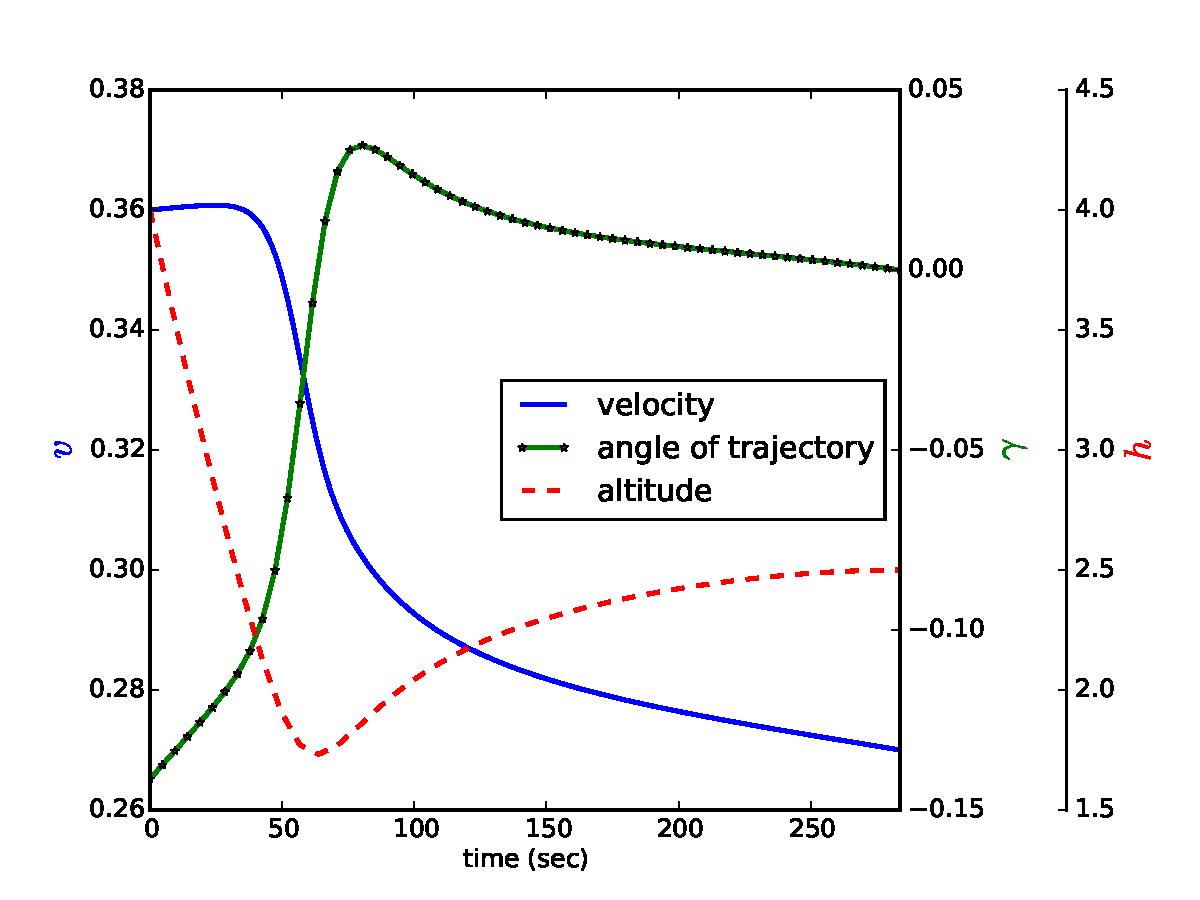
\includegraphics[width=\textwidth]{solutions.pdf}
\caption{The optimal path for reentry maneuver of spacecraft. The optimal path minimizes the heating of the spacecraft, and satisfies \eqref{eqn:reentry:full_system},\eqref{eqn:reentry:BCs}, and the terminal condition $H(T) = 0$.
}
\label{fig:reentry:solutions}
\end{figure}



\section*{Constructing an Initial Guess}
This nonlinear BVP is very sensitive, and requires an initial guess that is quite close to the solution.  
This is intuitively obvious: if the control is not aggressive, the spacecraft will fall back into space. 
If the control lasts too long, the craft will burn up on reentry. 

Since this is a sensitive problem, we will use a heuristic method to help us find a good initial guess.

Guess that $u = p_0\erf(p_1(p_2-t/T))$, where $p_0, p_1,$ and $p_2$ are unknown constants. 
We define an auxiliary problem to help us come up with a good initial guess for the original BVP. 
\begin{align}
\begin{split}
\dot{y_0} &= -s\rho y_0^2C_D(u) - \frac{g\sin(y_1)}{(1+y_2)^2},\\
\dot{y_1} &= s \rho y_0 C_L(u) + \frac{y_0 \cos(y_1)}{R(1+y_2)} - \frac{g \cos y_1}{y_0(1+y_2)^2},\\
\dot{y_2} &= \frac{y_0 \sin y_1}{R} ,\\
\dot{p_0} &= 0, \\
\dot{p_1} &= 0, \\
\dot{p_2} &= 0.
\end{split} \label{eqn:reentry:control_system_auxiliary}
\end{align}



The following code includes import statements, defines the parameters of the BVP, and creates functions for the drag coefficients. 
\begin{lstlisting}
from __future__ import division
from math import sin, cos
from scipy.special import erf
from scikits import bvp_solver 

R = 209
beta = 4.26
rho0 = 2.704e-3
g = 3.2172e-4
s = 26600	
T_init = 230

def C_d(u): 
	return 1.174 - 0.9*cos(u)

def C_l(u): 
	return 0.6*sin(u)
	
\end{lstlisting}

For the auxiliary problem, we code functions for the ode and for the boundary conditions. 
\begin{lstlisting}
def ode_auxiliary(x,y):
	u = y[3]*erf( y[4]*(y[5]-x/T_init) )
	rho = rho0*exp(-beta*R*y[2])
	out = array([-s*rho*y[0]**2*C_d(u) - g*sin(y[1])/(1+y[2])**2,
				  ( s*rho*y[0]*C_l(u) + y[0]*cos(y[1])/(R*(1 + y[2])) - 
				  g*cos(y[1])/(y[0]*(1+y[2])**2) ),
				  y[0]*sin(y[1])/R,
				  0,
				  0,
				  0		])
	return out
	
def bcs_auxiliary(ya,yb):
	# If the problem is defined on the interval [a,b], ya = y(a) and yb = y(b), 
	# ya[0] = y_0(a), etc.
	# bvp_solver will attempt to make each of the entries below zero in the 
	# numerical solution.
	
	out1 = array([ya[0]-.36,
				  ya[1]+8.1*pi/180,
				  ya[2]-4/R
				  ])
	out2 = array([yb[0]-.27,
				  yb[1],
				  yb[2]-2.5/R
				  ])
	return out1, out2

problem_auxiliary = bvp_solver.ProblemDefinition(num_ODE = 6,
										  num_parameters = 0,
										  num_left_boundary_conditions = 3,
										  boundary_points = (0., T_init),
										  function = ode_auxiliary,
										  boundary_conditions = bcs_auxiliary)
									
solution_auxiliary = bvp_solver.solve(problem_auxiliary,
								solution_guess = guess_auxiliary)
								
N = 240 # Number of subintervals
x_array = linspace(0,T_init,N+1)
y_array = solution_auxiliary(x_array)
	
\end{lstlisting}

\begin{figure}
\begin{minipage}[b]{.47\linewidth}
\centering
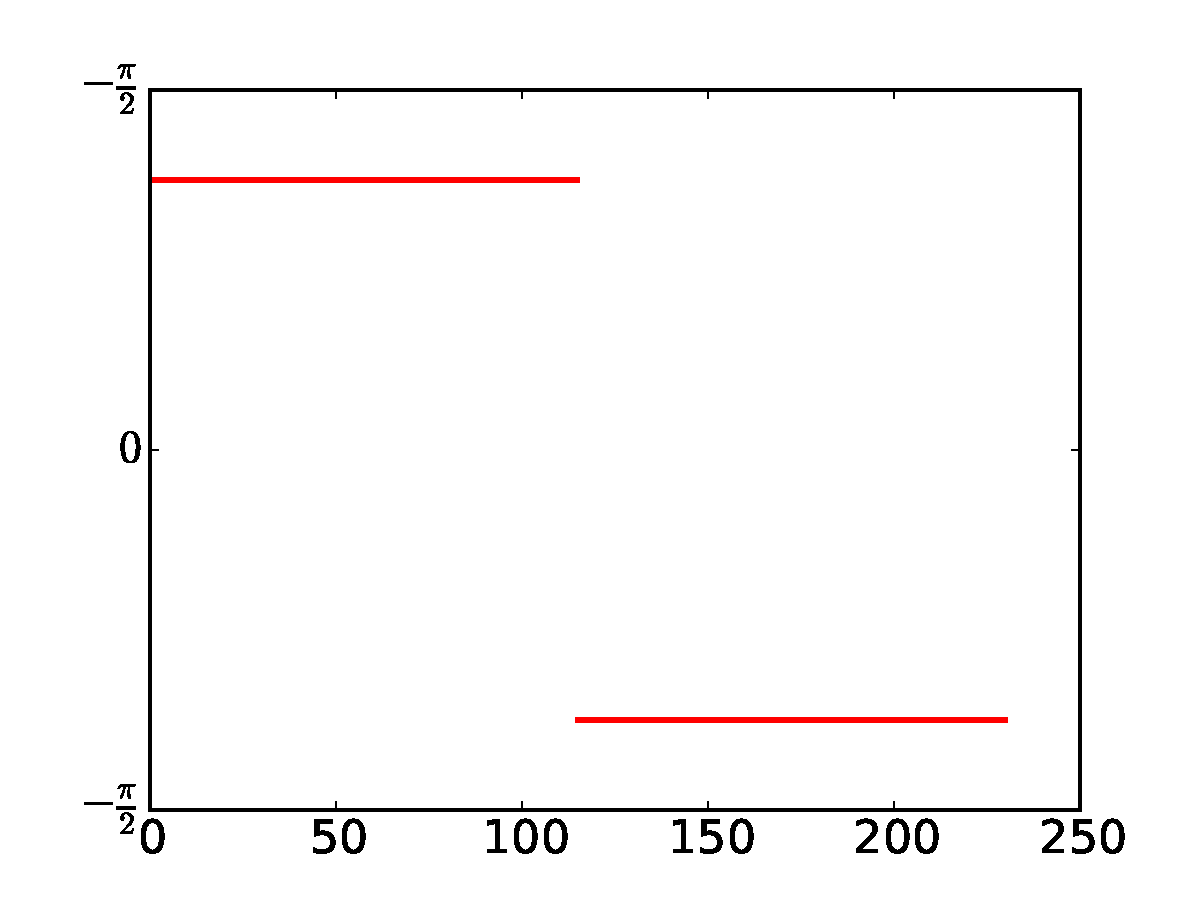
\includegraphics[width=\textwidth]{u_heuristic.pdf}
\caption*{Heuristic for the control $u$, provided by engineers. }
\end{minipage}
\hspace{0.5cm}
\begin{minipage}[b]{0.47\linewidth}
\centering
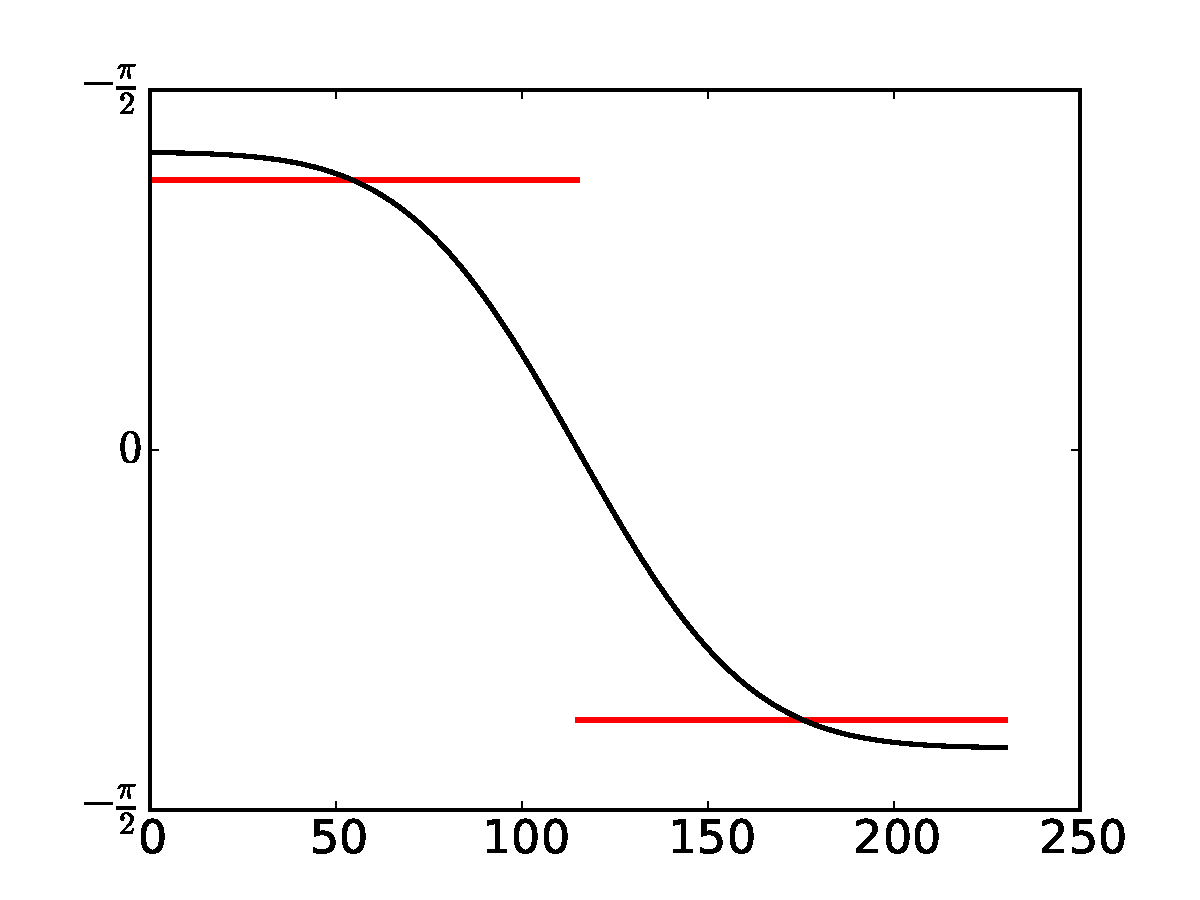
\includegraphics[width=\textwidth]{u_heuristic_smooth.pdf}
\caption*{A smooth initial approximation of the control.}
\end{minipage}
\caption{We construct a smooth estimate for the control $u$, by supposing the control has the form 
$u = p_0\erf(p_1(p_2-t/T))$ and estimating parameters $p_0, p_1, p_2$.}
\label{fig:reentry:estimate_u}
\end{figure}


\begin{problem}
	Write the function \li{guess_auxiliary} referenced in the code above. 
	This function provides an initial guess to \li{bvp_solver} for the auxiliary BVP described by  \eqref{eqn:reentry:control_system_auxiliary} and \eqref{eqn:reentry:BCs}.
	Use the heuristic data provided in Figure \ref{fig:reentry:estimate_u} to find good estimates of $p_0, p_1,$ and $p_2$. 
	Use Figure \ref{fig:reentry:solutions} to estimate the trajectories of $y_0, y_1,$ and $y_2$.
	Then run the code above to check that your initial guess is adequate. 
\end{problem}


\begin{problem}
	Write a function \li{ode} that implements the ODEs for the original control system along with the adjoint equations \eqref{eqn:reentry:full_system}. 
\end{problem}

Most BVP solvers require an equal number of differential equations and boundary conditions. 
Currently we have a free boundary value problem; there are 6 ODEs and 7 boundary conditions, and the length of the reentry maneuver, $T$, is still unknown. 
By making the transformation $x = t/T$, and letting $T$ by a dependent variable, the boundary value problem is now defined on the interval $(0,1)$ and can be supplemented with an additional ODE: 
\begin{align}
\begin{split}
	y' &= TH_{\lambda},\quad ' = \frac{d}{dx},\\
	\lambda' &= -TH_{y},\\
	T' &= 0. \label{eqn:reentry:full_system}
\end{split}	
\end{align}
Now the BVP has 7 ODEs and 7 boundary conditions, and thus has the form required by \li{bvp_solver}. 

\begin{problem}
Incorporate this change into the function \li{ode} written earlier. 
Also write a function \li{bcs} that implements the full set of boundary conditions. 
\end{problem}

Discuss how to construct an initial guess for the original BVP. Specifically, how should the adjoint variables be estimated?
\begin{problem}
	Adapt your previous code to solve the original, dimension seven BVP. You may want to look at the docstring of \li{bvp_solver.solve} to see more of its functionality.
	Plot the control $u$. How long does the reentry maneuver take? 
\end{problem}


% \begin{figure}
% \begin{minipage}[b]{.47\linewidth}
% \centering
% 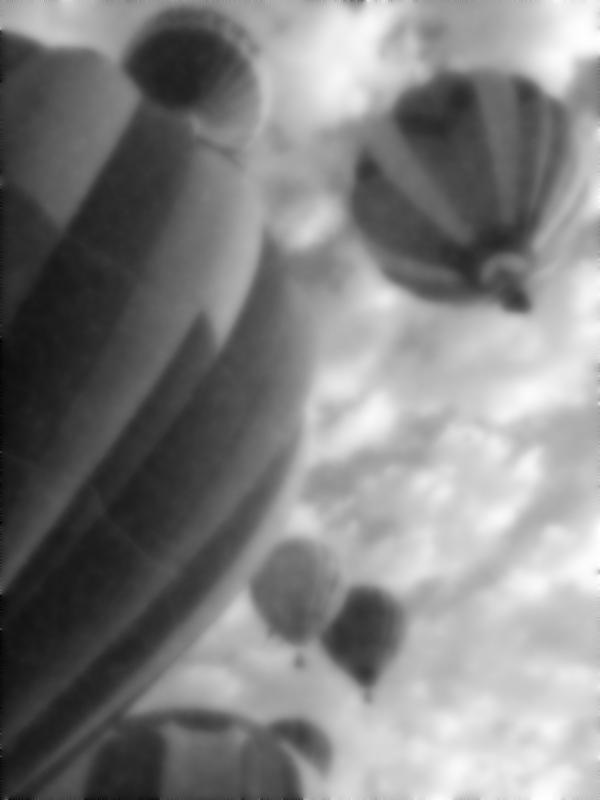
\includegraphics[width=\textwidth]{diffusion_denoised_baloons_resized_bw.jpg}
% \caption*{Initial diffusion-based approach}
% \end{minipage}
% \hspace{0.5cm}
% \begin{minipage}[b]{0.47\linewidth}
% \centering
% 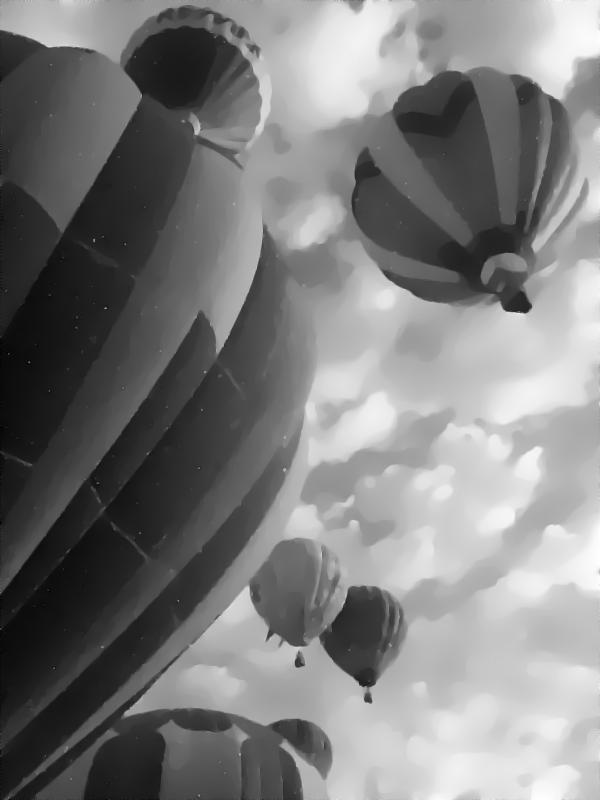
\includegraphics[width=\textwidth]{tv_denoised_baloons_resized_bw.jpg}
% \caption*{Total variation based approach}
% \end{minipage}
% \caption{The solutions of \eqref{tv_images:diffusion_flow} and \eqref{tv_images:tv_flow}, found using a first order Euler step in time and centered differences in space.}
% \label{fig:noise_compare_attempts}
% \end{figure}



% \begin{align}
% \begin{split}
% \end{split} \label{reentry:label}
% \end{align}
%
%
% \begin{problem}
%
% \begin{lstlisting}
% \end{lstlisting}
% \end{problem}


% \begin{figure}
% \centering
% 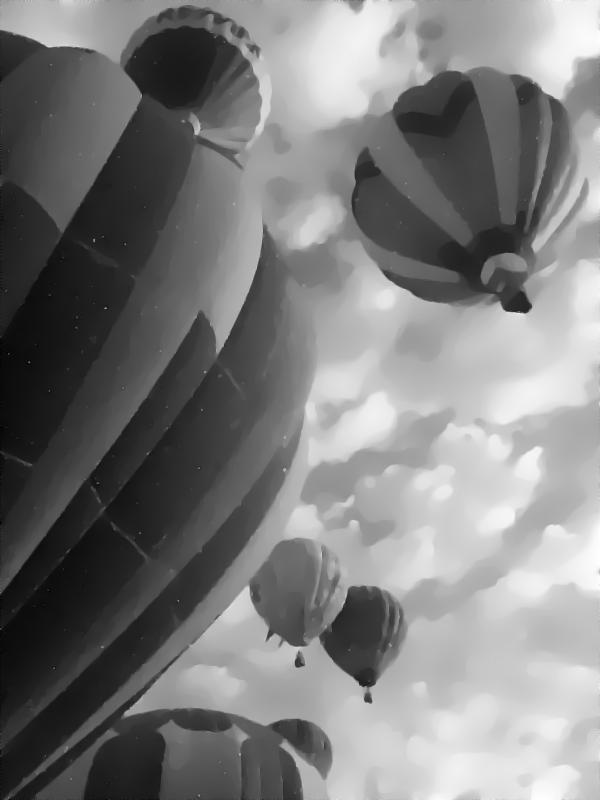
\includegraphics[width=6cm]{tv_denoised_baloons_resized_bw.jpg}
% \caption{The solution of \eqref{tv_images:diffusion_flow}, found using a first order Euler step in time and centered differences in space.}
% \label{fig:tv_image_denoised}
% \end{figure}







